%\documentclass[10pt,twocolumn,twoside]{IEEEtran}
%\documentclass[draftclsnofoot,onecolumn,12pt]{IEEEtran}
%\documentclass[draftclsnofoot,onecolumn,11pt,peerreview]{IEEEtran}
\documentclass[12pt]{article}
\usepackage{fullpage}
\usepackage{pgfplots}
\usepackage{subfigure}
\usepackage{tikz}

\usepackage{makeidx}

\usepackage[cmex10]{amsmath}
\usepackage{amsthm,amssymb,mathrsfs}
\usepackage{graphicx}
\usepackage{url}
\usepackage{cite}
%\usepackage{apacite}
%\usepackage{natbib}
\usepackage{lineno}
\usepackage{verbatim}
\usepackage{bm}
\usepackage{multirow}
\usepackage{booktabs}
\usepackage{amsthm}
\usepackage{array}
%\usepackage[usenames,dvipsnames]{color}
\usepackage{color,xcolor}
\usepackage{framed}
\usepackage{hyperref}
\definecolor{shadecolor}{gray}{0.9}
\newcommand*{\vertbar}{\rule[-0.75ex]{0.25pt}{2.5ex}}
\newcommand*{\horzbar}{\rule[.5ex]{2.5ex}{0.25pt}}

\begin{document}
\title{Solution for the Search Results Relevance Challenge}
\author{Chenglong~Chen}
\maketitle

\abstract{In the Search Results Relevance Challenge, we were asked to build a model to predict the relevance score of search results, given the searching queries, resulting product titles and product descriptions. This document describes our team's solution, which relies heavily on feature engineering and model ensembling.}

\section*{Personal details}
\begin{itemize}
\item Name: Chenglong Chen
\item Location: Guangzhou, Guangdong, China
\item Email: \url{c.chenglong@gmail.com}
\item Competition: Search Results Relevance\footnote{\url{https://www.kaggle.com/c/crowdflower-search-relevance}}
\end{itemize}

\newpage
\tableofcontents

\newpage
\section{Summary}
Our solution consisted of two parts: feature engineering and model ensembling. We had developed mainly three types of feature:
\begin{itemize}
\item counting features
\item distance features
\item TF-IDF features
\end{itemize}
Before generating features, we have found that it's helpful to process the text of the data with spelling correction, synonym replacement, and stemming. Model ensembling consisted of two main steps, Firstly, we trained model library using different models, different parameter settings, and different subsets of the features. Secondly, we generated ensemble submission from the model library predictions using bagged ensemble selection. Performance was estimated using cross validation within the training set. No external data sources were used in our winning submission. The flowchart of our method is shown in Figure \ref{fig:Flowchart}.

The best single model we have obtained during the competition was an XGBoost model with linear booster of Public LB score \textbf{0.69322} and Private LB score \textbf{0.70768}. Our final winning submission was a median ensemble of 35 best Public LB submissions. This submission scored \textbf{0.70807} on Public LB (our second best Public LB score) and \textbf{0.72189} on Private LB. \footnote{The best Public LB score was \textbf{0.70849} with corresponding Private LB score \textbf{0.72134}. It's a mean ensemble version of those 35 LB submissions.}

\begin{comment}
\begin{figure}[!htb]
\centering
\begin{tikzpicture}
\draw (-1.5,0) -- (1.5,0);
\draw (0,-1.5) -- (0,1.5);
\end{tikzpicture}
\end{figure}
\end{comment}
\begin{figure}[!htb]
\centering
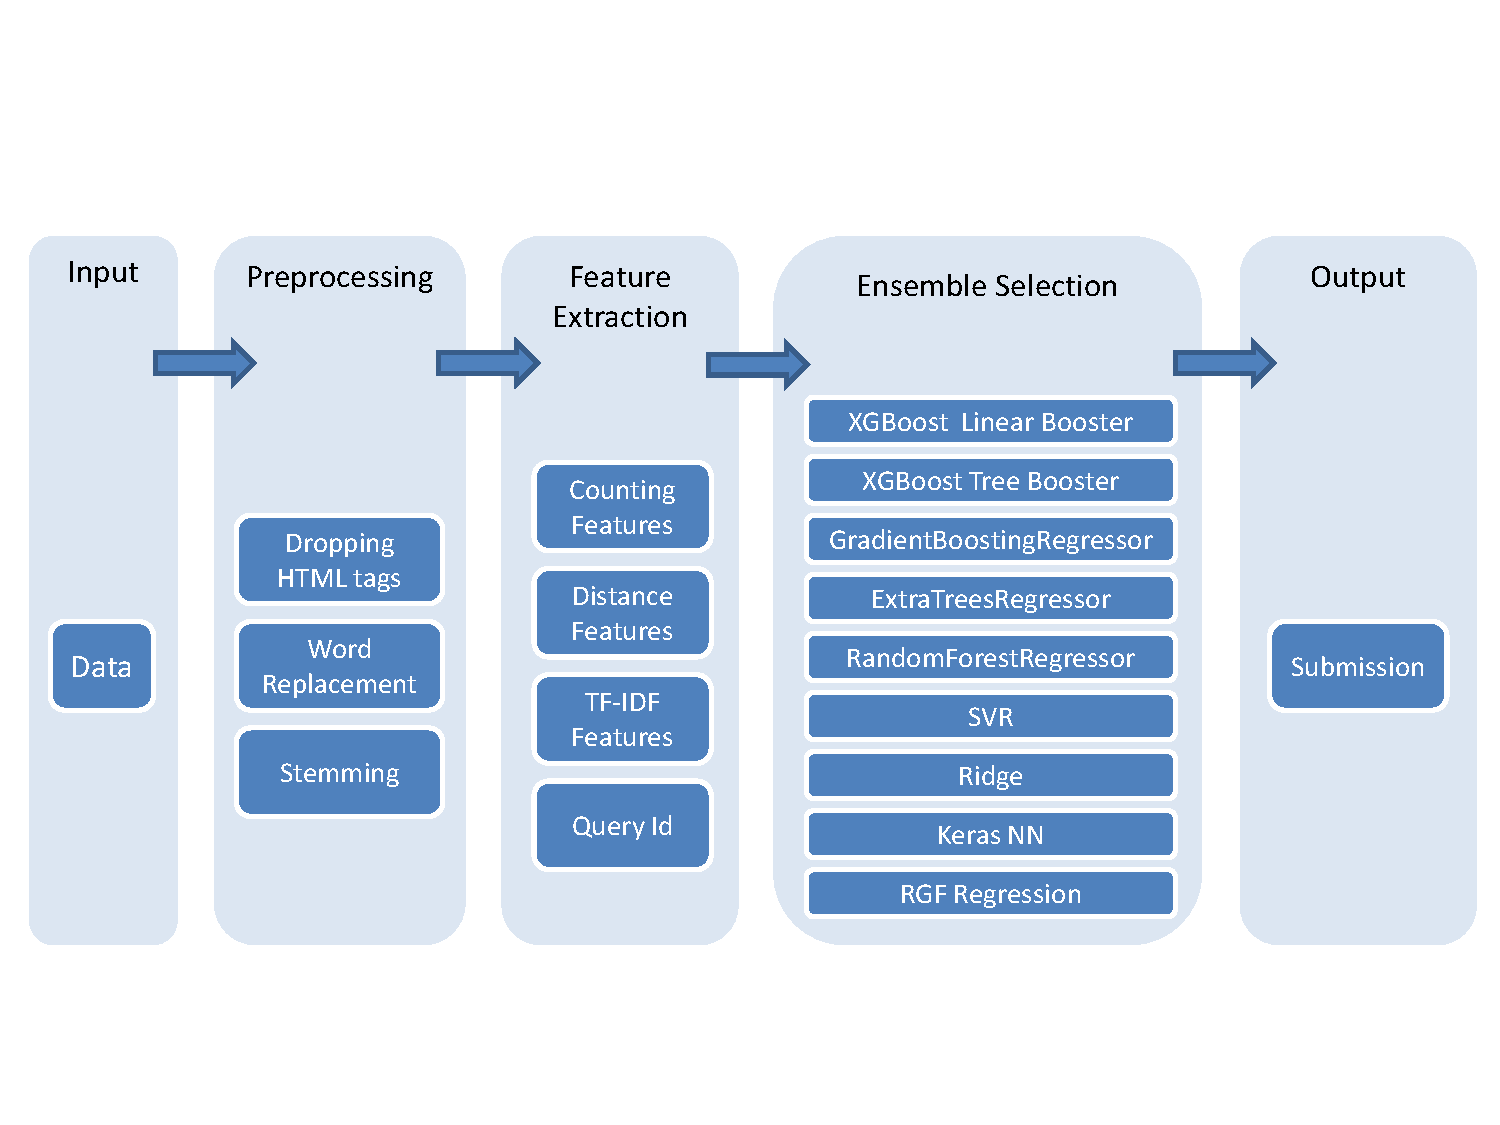
\includegraphics[width=0.9\textwidth]{./FlowChart.pdf}
\caption{The flowchart of our method.}
\label{fig:Flowchart}
\end{figure}

\section{Preprocessing}
A few steps were performed to cleaning up the text.
\subsection{Dropping HTML tags}
There are some noisy HTML tags in \texttt{product\_description} field, we used the library \texttt{bs4} to clean them up. It didn't bring much gain, but we have kept it anyway.

\subsection{Word Replacement}
We have created features similar as ``how many words of query are in product title'', so it's important to perform some word replacements, e.g., spelling correction and synonym replacement, to align those words with the same or similar meaning. By exploring the provided data, it seems CrowdFlower has already applied some word replacements in the searching results.

\subsubsection{Spelling Correction}
The misspellings we have identified are listed in Table \ref{tab:spelling_correction}. Note that this is by no means an exhaustive list of all the misspellings in the provided data. It is just the misspellings we have found while exploring the training data during the competition. This also applies to Table \ref{tab:synonym} and Table \ref{tab:Other}.
\begin{table}[!htb]
\centering
\caption{Spelling Correction}
\label{tab:spelling_correction}
\begin{tabular}{|c|c|}
\hline
\textcolor{red}{misspellings} & \textcolor{blue}{correction} \\
\hline\hline
\textcolor{red}{refrigirator} & \textcolor{blue}{refrigerator} \\
\textcolor{red}{rechargable} batteries & \textcolor{blue}{rechargeable} batteries \\
adidas \textcolor{red}{fragance} & adidas \textcolor{blue}{fragrance}\\
\textcolor{red}{assassinss} creed & \textcolor{blue}{assassins} creed\\
\textcolor{red}{rachel} ray cookware & \textcolor{blue}{rachael} ray cookware \\
donut \textcolor{red}{shoppe} k cups & donut \textcolor{blue}{shop} k cups \\
\textcolor{red}{extenal} hardisk 500 gb & \textcolor{blue}{external} hardisk 500 gb \\
\hline
\end{tabular}
\end{table}

\subsubsection{Synonym Replacement}
Table \ref{tab:synonym} lists out the synonyms we have found within the training data.
\begin{table}[!htb]
\centering
\caption{Synonym Replacement}
\label{tab:synonym}
\begin{tabular}{|c|c|}
\hline
synonyms & replacement\\
\hline\hline
child, kid & kid\\
bicycle, bike & bike\\
refrigerator, fridge, freezer & fridge\\
fragrance, perfume, cologne, eau de toilette & perfume\\
\hline
\end{tabular}
\end{table}


\subsubsection{Other Replacements}
Apart from the above two types of replacement, we also replace those words listed in Table \ref{tab:Other} to align them. \footnote{For a complete list of all the replacements, please refer to file \texttt{./Data/synonyms.csv} and variable \texttt{replace\_dict} in file \texttt{./Code/Feat/nlp\_utils.py}}
\begin{table}[!htb]
\centering
\caption{Other Replacement}
\label{tab:Other}
\begin{tabular}{|c|c|}
\hline
original & replacement\\
\hline\hline
nutri system & nutrisystem\\
soda stream & sodastream\\
playstation & ps\\
ps 2 & ps2\\
ps 3 & ps3\\
ps 4 & ps4\\
coffeemaker & coffee maker\\
k-cup & k cup\\
4-ounce & 4 ounce\\
8-ounce & 8 ounce\\
12-ounce & 12 ounce\\
ounce & oz\\
hardisk & hard drive\\
hard disk & hard drive\\
harley-davidson & harley davidson\\
harleydavidson & harley davidson\\
doctor who & dr who\\
levi strauss & levis\\
mac book & macbook\\
micro-usb & micro usb\\
video games & videogames\\
game pad & gamepad\\
western digital & wd\\
\hline
\end{tabular}
\end{table}

\subsection{Stemming}
We also performed stemming before generating features (e.g., counting features and BOW/TF-DF features) with Porter stemmer or Snowball stemmer from NLTK package (i.e., \texttt{nltk.stem.PorterStemmer()} and \texttt{nltk.stem.SnowballStemmer()}).

\section{Feature Extraction/Selection}
Before proceeding to describe the features, we first introduce some notations. We use tuple $(q_i, t_i, d_i)$ to denote the $i$-th sample in \texttt{train.csv} or \texttt{test.csv}, where $q_i$ is the \texttt{query}, $t_i$ is the \texttt{product\_title}, and $d_i$ is the \texttt{product\_description}. For \texttt{train.csv}, we further use $r_i$ and $v_i$ to denote \texttt{median\_relevance} and \texttt{relevance\_variance}\footnote{This is actually the standard deviation (std).}, respectively. We use function $\text{ngram}(s, n)$ to extract string/sentence $s$'s $n$-gram (splitted by whitespace), where $n\in\{1,2,3\}$ if not specified. For example
\[
\text{ngram}(\text{bridal shower decorations}, 2) = [\text{bridal shower}, \text{shower decorations}]\footnote{Note that this is a list (e.g., \texttt{list} in Python), not a set (e.g., \texttt{set} in Python).}
\]

\textbf{All the features are extracted for each run (i.e., repeated time) and fold (used in cross-validation and ensembling), and for the entire training and testing set (used in final model building and generating submission).}

In the following, we will give a description of the features we have developed during the competition, which can be roughly divided into four types.
\subsection{Counting Features}
\label{subsec:Counting_Features}
We generated counting features for $\{q_i, t_i, d_i\}$. For some of the counting features, we also computed the ratio following the suggestion from Owen Zhang \cite{owen}.

The file to generate such features is provided as \textbf{genFeat\_counting\_feat.py}.
\subsubsection{Basic Counting Features}
\begin{itemize}
\item \textbf{Count of $n$-gram}\\
count of $\text{ngram}(q_i, n)$, $\text{ngram}(t_i, n)$, and $\text{ngram}(d_i, n)$.
\item \textbf{Count \& Ratio of Digit}\\
count \& ratio of digits in $q_i$, $t_i$, and $d_i$.
\item \textbf{Count \& Ratio of Unique $n$-gram}\\
count \& ratio of unique $\text{ngram}(q_i, n)$, $\text{ngram}(t_i, n)$, and $\text{ngram}(d_i, n)$.
\item \textbf{Description Missing Indicator}\\
binary indicator indicating whether $d_i$ is empty.
\end{itemize}

\subsubsection{Intersect Counting Features}
\begin{itemize}
\item \textbf{Count \& Ratio of $a$'s $n$-gram in $b$'s $n$-gram}\\
Such features were computed for all the combinations of $a\in\{q_i, t_i, d_i\}$ and $b\in\{q_i, t_i, d_i\}$ ($a\neq b$).
\end{itemize}

\subsubsection{Intersect Position Features}
\begin{itemize}
\item \textbf{Statistics of Positions of $a$'s $n$-gram in $b$'s $n$-gram}\\
For those intersect $n$-gram, we recorded their positions, and computed the following statistics as features.
\begin{itemize}
        \item minimum value (0\% quantile)
        \item median value (50\% quantile)
        \item maximum value (100\% quantile)
        \item mean value
        \item standard deviation (std)
\end{itemize}
\item \textbf{Statistics of Normalized Positions of a's $n$-gram in b's $n$-gram}\\
These features are similar with above features, but computed using positions normalized by the length of $a$.
\end{itemize}

\subsection{Distance Features}
\label{subsec:Distance_Features}
Jaccard coefficient
\begin{equation}
\text{JaccardCoef}(A, B) = \frac{|A\cap{B}|}{|A\cup{B}|}
\end{equation}
and Dice distance
\begin{equation}
\text{DiceDist}(A, B) = \frac{2|A\cap{B}|}{|A|+|B|}
\end{equation}
are used as distance metrics, where $A$ and $B$ denote two sets respectively. For each distance metric, two types of features are computed.

The file to generate such features is provided as \textbf{genFeat\_distance\_feat.py}.
\subsubsection{Basic Distance Features}
The following distances are computed as features
\begin{itemize}
\item $D(\text{ngram}(q_i, n), \text{ngram}(t_i, n))$
\item $D(\text{ngram}(q_i, n), \text{ngram}(d_i, n))$
\item $D(\text{ngram}(t_i, n), \text{ngram}(d_i, n))$
\end{itemize}
where $D(\cdot, \cdot)\in\{\text{JaccardCoef}(\text{set}(\cdot), \text{set}(\cdot)), \text{DiceDist}(\text{set}(\cdot), \text{set}(\cdot))\}$, and $\text{set}(\cdot)$ converts the input to a set.

\subsubsection{Statistical Distance Features}
\label{subsubsec:Statistical_Distance_Features}
These features are inspired by Gilberto Titericz and Stanislav Semenov's winning solution \cite{Otto_1st} to Otto Group Product Classification Challenge on Kaggle. They are computed for \texttt{product\_title} and \texttt{product\_description}, respectively. Take \texttt{product\_title} for examples. They are computed in the following steps.
\begin{enumerate}
\item group the samples by \texttt{median\_relevance} and (\texttt{query}, \texttt{median\_relevance}).
\begin{equation}
G_r = \{i \,|\, r_i = r\}
\end{equation}
\begin{equation}
G_{q,r} = \{i \,|\, q_i = q, r_i = r\}
\end{equation}
where $q\in{\{q_i\}}$ (i.e., all the unique \texttt{query}) and $r\in{\{1,2,3,4\}}$.
\item compute distance between each sample and all the samples in each \texttt{median\_relevance} level. Note that we excluded the current sample being considered when computing the distance. For $G_{q,r}$, we considered the group with same query as the current sample.
\begin{equation}
S_{i,r,n} = \{D(\text{ngram}(t_i, n), \text{ngram}(t_j, n)) \,|\, j \in{G_r}, j \neq i \}
\end{equation}
\begin{equation}
SQ_{i,r,n} = \{D(\text{ngram}(t_i, n), \text{ngram}(t_j, n)) \,|\, j \in{G_{q_i,r}}, j \neq i \}
\end{equation}
where $r\in{\{1,2,3,4\}}$ and $D(\cdot, \cdot)\in\{\text{JaccardCoef}(\cdot, \cdot), \text{DiceDist}(\cdot, \cdot)\}$.
\item for $S_{i,r,n}$ and $SQ_{i,r,n}$, respectively, compute statistics such as
    \begin{itemize}
        \item minimum value (0\% quantile)
        \item median value (50\% quantile)
        \item maximum value (100\% quantile)
        \item mean value
        \item standard deviation (std)
        \item more can be added, e.g., moment features and other quantiles
    \end{itemize}
    as features.
\end{enumerate}

\subsection{TF-IDF Based Features}
We extracted various TF-IDF features and the corresponding dimensionality reduction version via SVD (i.e., LSA). We also computed the (basic) cosine similarity and statistical cosine similarity.
\subsubsection{Basic TF-IDF Features}
\label{subsubsec:Basic_TFIDF_Features}
The file to generate such features is provided as \textbf{genFeat\_basic\_tfidf\_feat.py}.
\begin{itemize}
\item \textbf{TF-IDF Features}\\
We extracted TF-IDF features from $\{q_i, t_i, d_i\}$, respectively. We considered unigram \& bigram \& trigram (in Sklearn's \texttt{TfidfVectorizer}, set \texttt{ngram\_range}=(1,3).)
\begin{itemize}
\item \textbf{Common Vocabulary}\\
Note that to ensure the TF-IDF feature vectors of $\{q_i, t_i, d_i\}$ are projected into the same vector space, we first concatenated $\{q_i, t_i, d_i\}$, and then fit a TF-IDF transformer to obtain the common vocabulary. We then used this common vocabulary to generate TF-IDF features for $\{q_i, t_i, d_i\}$, respectively.
\item \textbf{Individual Vocabulary}\\
We fit TF-IDF transformer for $\{q_i, t_i, d_i\}$, separately, with individual vocabulary.
\end{itemize}
\item \textbf{Basic Cosine Similarity}\\
With previous generated TF-IDF features (using common vocabulary), we computed the cosine similarity of
\begin{itemize}
\item $q_i$ and $t_i$
\item $q_i$ and $d_i$
\item $t_i$ and $d_i$
\end{itemize}
\item \textbf{Statistical Cosine Similarity}\\
Since cosine similarity is a distance metric, we also computed statistical cosine similarity as in Sec. \ref{subsubsec:Statistical_Distance_Features}.
\item \textbf{SVD Reduced Features}\\
We performed SVD to the above TF-IDF features to obtain a dimension reduced feature vector. Such reduced version was mostly used together with non-linear models, e.g., random forest and gradient boosting machine.
\begin{itemize}
\item \textbf{Common SVD}\\
We first concatenated the TF-IDF vectors of $\{q_i, t_i, d_i\}$ (using common vocabulary), and fit a SVD transformer.
\item \textbf{Individual SVD}\\
We fit a SVD transformer for TF-IDF vectors of $\{q_i, t_i, d_i\}$, separately.
\end{itemize}
\item \textbf{Cosine Similarity Based on SVD Reduced Features}\\
We computed cosine similarity based on SVD reduced features (using common SVD).
\item \textbf{Statistical Cosine Similarity Based on SVD Reduced Features}\\
We computed statistical cosine similarity based on SVD reduced features.
\end{itemize}
\subsubsection{Cooccurrence TF-IDF Features}
\label{subsubsec:Cooccurrence_TFIDF_Features}
We extracted TF-IDF for cooccurrence terms between
\begin{itemize}
\item \texttt{query} unigram/bigram and \texttt{product\_title} unigram/bigram
\item \texttt{query} unigram/bigram and \texttt{product\_description} unigram/bigram
\item \texttt{query} id (\texttt{qid}) and \texttt{product\_title} unigram/bigram
\item \texttt{query} id (\texttt{qid}) and \texttt{product\_description} unigram/bigram
\end{itemize}

We give an example to explain what's cooccurrence terms. Consider sample with \texttt{id} = 54 in \texttt{train.csv} (see Table \ref{tab:sample_id54}). For this sample, we have (after converting to lowercase)
\begin{table}[!htb]
\centering
\caption{One sample in \texttt{train.csv}}
\label{tab:sample_id54}
\begin{tabular}{|c|c|c|}
\hline
\texttt{id} & \texttt{query} & \texttt{product\_title} \\
\hline
54 & silver necklace & fremada sterling silver freeform necklace\\
\hline
\end{tabular}
\end{table}
\begin{itemize}
\item cooccurrence terms for \texttt{query} unigram and \texttt{product\_title} unigram is\\
$[$silver fremada, silver sterling, silver silver, silver freeform, silver necklace, necklace fremada, necklace sterling, necklace silver, necklace freeform, necklace necklace$]$
\item cooccurrence terms for \texttt{query} bigram and \texttt{product\_title} unigram is\\
$[$silver necklace fremada, silver necklace sterling, silver necklace silver, silver necklace freeform, silver necklace necklace$]$
\end{itemize}
We have found that such features are very useful for linear model (e.g., XGBoost with linear booster). We suspect it is because these features add nonlinearity to the model. We also performed SVD to such features though we haven't found much gain using the corresponding SVD features.

The file to generate such features is provided as \textbf{genFeat\_cooccurrence\_tfidf\_feat.py}.


\subsection{Other Features}
\subsubsection{Query Id}
one-hot encoding of the \texttt{query} (generated via \texttt{genFeat\_id\_feat.py})

\subsection{Feature Selection}
For feature selection, we adopted the idea of ``untuned modeling'' as used in Marios Michailidis and Gert Jacobusse's 2nd place solution \cite{malware_2nd} to Microsoft Malware Classification Challenge on Kaggle. The same model is always used to perform cross validation on a (combined) set of features to test whether it improves the
score compared to earlier feature sets. For features of high dimension (denoted as ``High''), e.g., feature set including raw TF-IDF features, we used XGBoost with linear booster (MSE objective); otherwise, we used \texttt{ExtraTreesRegressor} in Sklearn for features of low dimension (denoted as ``Low'').

Note that with ensemble selection, one can train model library with various feature set and rely on ensemble selection to pick out the best ensemble within the model library. However, feature selection is still helpful. Using the above feature selection method, one can first identified some (possible) well performed feature set, and then trained model library with it. This helps to reduce the computation burden to some extent.

\section{Modeling Techniques and Training}
\subsection{Cross Validation Methodology}
\subsubsection{The Split}
Early in the competition, we have been using \texttt{StratifiedKFold} on \texttt{median\_relevance} or \texttt{query} with $k = 5$ or $k = 10$, but there was a large gap between our CV score and Public LB score. We then changed our CV method to \texttt{StratifiedKFold} on \texttt{query} with $k = 3$, and used \emph{each 1 fold as training set} and \emph{the rest 2 folds as validation set}. This is to mimic the training-testing split of the data as pointed out by Kaggler @Silogram. With this strategy, our CV score tended to be more correlated with the Public LB score (see Table \ref{CV_LB}).
\subsubsection{Following the Same Logic}
Since this is an NLP related competition, it's common to use TF-IDF features. We have seen a few people fitting a TF-IDF transformer on the stacked training and testing set, and then transforming the training and testing set, respectively. They then use such feature vectors (\textbf{they are fixed}) for cross validation or grid search for the best parameters. They call such method as semi-supervised learning. In our opinion, if one is taking such method, he should refit the transformer using only the whole training set in CV, following the same logic.

On the other hand, if one fit the transformer on the training set (for the final model building), then in CV, he should also refit the transformer on the training fold only. This is the method we used. Not only for TF-IDF transformer, but also for other transformations, e.g., normalization and SVD, one should make sure he is following the same logic in both CV and the final model building.

\begin{table}[t]
\centering
\caption{CV score and LB score}
    \label{CV_LB}
\begin{tabular}{|c|c|c|c|c|c|}
\hline
CV Mean   & CV Std  &  Public LB  &    Private LB   &   CV Method   &  Repeated Time\\
\hline\hline
0.642935  & 0.003694  &  0.63773   &  0.66185  & 3-fold CV     &     10\\
0.661263  & 0.008021  &  0.66529   &  0.69208 &  3-fold CV     &     3\\
0.664184  & 0.008027  &  0.66775   &  \textcolor{red}{0.69596} &  3-fold CV    &      3\\
0.668797  & 0.008394  &  0.67020   &  0.69509 &  3-fold CV    &      3\\
0.669313  & 0.007969  &  0.67166   &  0.69267 &  3-fold CV    &      3\\
\textcolor{red}{0.669399}  & 0.006669  &  \textcolor{red}{0.67275}   &  0.69135 &  3-fold CV    &      3\\
\hline
\end{tabular}
\end{table}

\subsection{Model Objective and Decoding Method}
In this competition, submissions are scored based on the \emph{quadratic weighted kappa}, which measures the agreement between two ratings. This metric typically varies from 0 (random agreement between raters) to 1 (complete agreement between raters).

Results have 4 possible ratings, $\{1,2,3,4\}$. Each search record is characterized by a tuple $(e_a,e_b)$, which corresponds to its scores by Rater A (human) and Rater B (predicted). The quadratic weighted kappa is calculated as follows. First, an $N\times{N}$ histogram matrix $O$ is constructed, such that $O_{i,j}$ corresponds to the number of search records that received a rating $i$ by A and a rating $j$ by B. An $N\times{N}$ matrix of weights, $w$, is calculated based on the difference between raters' scores:
\begin{equation}
w_{i,j} = \frac{(i-j)^2}{(N-1)^2}
\end{equation}
An $N\times{N}$ histogram matrix of expected ratings, $E$, is calculated, assuming that there is no correlation between rating scores. This is calculated as the outer product between each rater's histogram vector of ratings, normalized such that $E$ and O have the same sum.

From these three matrices, the quadratic weighted kappa is calculated as:
\begin{equation}
\kappa = 1 - \frac{\sum_{i,j}w_{i,j}O_{i,j}}{\sum_{i,j}w_{i,j}E_{i,j}}
\end{equation}

\subsubsection{Classification}
\label{subsubsec:Classification}
Since the relevance score is in $\{1,2,3,4\}$, it is straightforward to apply multi-classification to the problem (using softmax loss). To convert the raw prediction (i.e., probabilities of four classes) to a single integer score, we can set it to the class label with the highest probability (i.e., \texttt{argmax}). However, we can achieve better score via the following strategy.
\begin{enumerate}
\item convert the four probabilities to a score via: $s = \sum_{i}iP_i$, i.e., weighted sum of the four probabilities.
\item calculate the pdf/cdf of each \texttt{median\_relevance} level, 1 is about $7.6\%$, $1+2$ is about $22\%$, $1+2+3$ is about $40\%$, and $1+2+3+4$ is $100\%$.
\item rank the raw prediction in an ascending order.
\item set the first $7.6\%$ to 1, $7.6\%-22\%$ to 2, $22\%-40\%$ to 3, and the rest to 4.
\end{enumerate}
In CV, the pdf/cdf is calculated using training fold only, and in final model training, it is computed using the whole training data.

This also applies to One-Against-All (OAA) classification, e.g., \texttt{LogisticRegression} in Sklearn.

\subsubsection{Regression}
Classification doesn't take into account the weight $w_{i,j}$ in $\kappa$, and the magnitude of the rating. With $w_{i,j}$'s form, it is convincing to apply regression (with mean-squared-error, MSE) to predict the relevance score. In prediction phase, we can convert the raw prediction score to $\{1,2,3,4\}$ following step 2-4 as in Sec. \ref{subsubsec:Classification}.

It turns out that MSE is the best objective among all the alternatives we have tried during the competition. For this reason, we mostly used regression to predict \texttt{median\_relevance}.

\subsubsection{Pairwise Ranking}
We have tried pairwise ranking (LambdaMart) within XGBoost, but didn't obtain acceptable performance (it was worse than softmax).

\subsubsection{Oridinal Regression}
We have also tried to treat the task as an ordinal regression problem, and have implemented the following two methods: EBC and COCR (and the corresponding decoding method). It turned out COCR has superior performance than EBC, but is on a similar edge with softmax.
\begin{itemize}
\item \textbf{Extended Binary Classification (EBC)}\\
This method is implemented within the XGBoost framework using customized objective. The objective and the corresponding decoding method of this method are in file \texttt{./Code/Model/utils.py}: \texttt{ebcObj} and \texttt{applyEBCRule}, respectively. For details of the EBC method, please refer to \cite{ebc}.
\item \textbf{Cost-sensitive Ordinal Classification via Regression (COCR)}\\
This method is implemented within the XGBoost framework using customized objective too. The objective and the corresponding decoding method of this method are in file \texttt{./Code/Model/utils.py}: \texttt{cocrObj} and \texttt{applyCOCRRule}, respectively. For details of the COCR method, please refer to \cite{cocr}.
\end{itemize}

\subsubsection{Softkappa}
Wse have tried to maximize $\kappa$ directly. To that goal, we re-write it in a soft-version using class probabilities.\footnote{Due to time and space constraints, we are not able to provide the detailed derivation in this version.} The objective is in file \texttt{./Code/Model/utils.py}: \texttt{softkappaObj}. The decoding method is the same as softmax and the performance is similar.

\subsection{Sample Weighting}
We are provided with the variance of the relevance scores given by raters. Such variance can be seem as a measure of the confidence of the ratings, and utilized to weight each sample. We have tried to weight the samples according to their variance, and it gives about 0.003 improvement. We have found the following weighting strategy works well in our models
\begin{equation}
w_i = \frac{1}{2}(1 + \frac{\hat{v}_m - \hat{v}_i}{\hat{v}_m})=1-\frac{\hat{v}_i}{2\hat{v}_m}
\end{equation}
where $\hat{v}_i = \sqrt{v_i}$ and $\hat{v}_m = \max_{i} \hat{v}_i$.

Most of our models (see Table \ref{tab:Model_Library}) used weighted data, and a few didn't as to
\begin{itemize}
\item generate diverse predictions for the ensemble;
\item sample weighting is not supported, e.g., \texttt{Lasso} in Sklearn.
\end{itemize}

\subsection{Ensemble Selection}
For the ensemble, we use bagged ensemble selection \cite{ensemble_selection}. One interesting feature of ensemble selection is its ability to build an ensemble optimized to an arbitrary metric, e.g., quadratic weighted kappa used in this competition. We have also made some modifications to the original algorithm. Firstly, the model library is built with parameters of each model guided by a parameter searching algorithm. Secondly, model weight optimization is allowed in the procedure of ensemble selection. Thirdly, we used random weight for ensembling model similar as \texttt{ExtraTreesRegressor}. In the following, we will detail our ensemble methodology.

\subsubsection{Model Library Building via Guided Parameter Searching}
Ensemble selection needs a model library contains lots (hundreds or thousands) of models trained used different algorithm (e.g., XGBoost or NN, see Table \ref{tab:Model_Library} for the algorithms we used) or different parameters (how may trees/layers/hidden units) or different feature sets. For each algorithm, we specified a parameter space, and used TPE method \cite{hyperopt} in Hyperopt package \cite{hyperopt_url} for parameter searching. It not only find the best parameter setting for each algorithm, but also create a model library with various parameter settings guided or provided by Hyperopt.

During parameter searching, we trained a model with each parameter setting on training fold for each run and each fold in cross-validation, and saved the rank of the prediction of the validation fold to disk. Note that such rank was obtained using the corresponding decoding method as in step 2-4 of Sec. \ref{subsubsec:Classification}. They were used in ensemble selection to find the best ensemble. We also trained a model with the same parameter setting on the whole training set, and saved the rank of the prediction of the testing set. Such rank predictions were used for generating the final ensemble submission.
\begin{table}[t]
\centering
\caption{Model Library}
    \label{tab:Model_Library}
\begin{tabular}{|c|c|c|c|c|}
\hline
Package   & \multicolumn{2}{c|}{Model}    & Feature & Weighting\\
\hline\hline
\multirow{8}*{XGBoost}  & \multirow{4}*{\texttt{gblinear}}  &  MSE & \multirow{4}*{High/Low}& \multirow{4}*{Yes}\\ \cline{3-3}
 &   &    COCR & &\\ \cline{3-3}
  &   &  Softmax  & &\\ \cline{3-3}
  &   &  Softkappa & &\\ \cline{3-3}
\cline{2-5}
  & \multirow{4}*{\texttt{gbtree}}  &  MSE  & \multirow{4}*{Low}& \multirow{4}*{Yes}\\ \cline{3-3}
 &   &    COCR & &\\ \cline{3-3}
  &   &  Softmax & &\\ \cline{3-3}
  &   &  Softkappa & &\\ \cline{3-3}
\hline
\multirow{7}*{Sklearn} & \multicolumn{2}{c|}{\texttt{GradientBoostingRegressor}} & Low & Yes\\ \cline{2-5}
  & \multicolumn{2}{c|}{\texttt{ExtraTreesRegressor}}      & Low & Yes\\ \cline{2-5}
  & \multicolumn{2}{c|}{\texttt{RandomForestRegressor}} & Low & Yes\\ \cline{2-5}
  & \multicolumn{2}{c|}{\texttt{SVR}}                            & Low & Yes\\ \cline{2-5}
  & \multicolumn{2}{c|}{\texttt{Ridge}}                & High/Low & Yes\\ \cline{2-5}
  & \multicolumn{2}{c|}{\texttt{Lasso}}                 & High/Low & No\\ \cline{2-5}
  & \multicolumn{2}{c|}{\texttt{LogisticRegression}}   & High/Low & No\\ \hline
Keras & \multicolumn{2}{c|}{NN Regression}                         & Low & No  \\ \hline
RGF & \multicolumn{2}{c|}{Regression}                              & Low  & No  \\ \hline
\end{tabular}
\end{table}
\subsubsection{Model Weight Optimization}
In the original ensemble selection algorithm, the model is added to the ensemble with hard weight 1. However, this is not guaranteed for best performance. We have modified it to allow weight optimized for each model when adding to the ensemble. The weight is optimized with Hyeropt too. This gives better performance than hard weight 1 in our preliminary comparison.

\subsubsection{Randomized Ensemble Selection}
The final method we used to generate the winning solution is actually without model weight optimization. On the contrary, we replaced weight optimization with \textbf{random weight}. This is inspired by the \texttt{ExtraTreesRegressor} to reduce the model variance (or the risk of overfitting). Figure \ref{fig:CV_Public_Private} shows the CV mean, Public LB, and Private LB scores of our 35 best Public LB submissions generated with this method. As shown, CV score is correlated with the Public LB and Private LB, while it's more correlated with the latter. As time went by, we have trained more and more different models, which turned out to be helpful for ensemble selection in both CV and Private LB (as shown in Figure \ref{fig:CV_Public_Private}). Finally, the winning solution that scored \textbf{0.70807} on Public LB and \textbf{0.72189} on Private LB is just a median ensemble of these 35 best Public LB submissions.

\begin{figure}[t]
\centering
\begin{tikzpicture}
\begin{axis}[
  xmin=0,
  xmax=36,
  %xtick={0,5,...,35},
  %xticklabel=$\pgfmathprintnumber{\tick}$,
  xtick=\empty,
  ylabel=$\kappa$,
  xlabel=$\longrightarrow \text{Time} \longrightarrow$,
  grid=major,
  grid style={dashed},
  legend columns=3,
legend style={at={(0.5,1.05)},anchor=south}
  ]
\pgfplotstableread{35lb_subs.txt}\loadedtable
\addplot +[error bars/.cd,
y dir=both,y explicit,
error mark=-] table[x index=0,y index=1,y error index=2,header=false] {\loadedtable};
\addplot +[smooth] table[x index=0,y index=3,header=false] {\loadedtable};
\addplot +[smooth] table[x index=0,y index=4,header=false] {\loadedtable};
\legend{%
CV mean,%
Public LB,%
Private LB}
\end{axis}
\end{tikzpicture}
\caption{CV mean, Public LB, and Private LB scores of our 35 best Public LB submissions generating with randomized ensemble selection. One standard deviation of the CV score is plotted via error bar.}
\label{fig:CV_Public_Private}
\end{figure}

\section{Code Description}
The implementation is organized in the following three parts.

\subsection{Setting}
\begin{itemize}
\item \textbf{param\_config.py}: This file provides parameter configurations for the project.
\end{itemize}

\subsection{Feature}
All the files are in the folder \texttt{./Code/Feat}.
\begin{itemize}
\item \textbf{ngram.py}: This file provides functions to compute n-gram \& n-term.
\item \textbf{replacer.py}: This file provides functions to perform synonym \& antonym replacement. Such functions are adopted from \cite{NLTK_Cookbook} (Chapter 2, Page 39-43.)
\item \textbf{nlp\_utils.py}: This file provides functions to perform NLP task, e.g., TF-IDF and POS tagging.
\item \textbf{feat\_utils.py}: This file provides utils for generating features.
\item \textbf{preprocess.py}: This file preprocesses data.
\item \textbf{gen\_info.py}: This file generates the following info for each run and fold, and for the entire training and testing set.
        \begin{enumerate}
            \item training and validation/testing data
            \item sample weight
            \item cdf of the \texttt{median\_relevance}
            \item the group info for pairwise ranking in XGBoost
        \end{enumerate}
\item \textbf{gen\_kfold.py}: This file generates the \texttt{StratifiedKFold} sample indices which will be kept fixed in \textbf{ALL} the following model building parts.
\item \textbf{genFeat\_id\_feat.py}: This file generates the following features for each run and fold, and for the entire training and testing set.
    \begin{enumerate}
    \item one-hot encoding of query ids (qid)
    \end{enumerate}
\item \textbf{genFeat\_counting\_feat.py}: This file generates the counting features described in Sec. \ref{subsec:Counting_Features} for each run and fold, and for the entire training and testing set.
\item \textbf{genFeat\_distance\_feat.py}: This file generates the distance features described in Sec. \ref{subsec:Distance_Features} for each run and fold, and for the entire training and testing set.
\item \textbf{genFeat\_basic\_tfidf\_feat.py}: This file generates the basic TF-IDF features described in Sec. \ref{subsubsec:Basic_TFIDF_Features} for each run and fold, and for the entire training and testing set.
\item \textbf{genFeat\_cooccurrence\_tfidf\_feat.py}: This file generates the cooccurrence TF-IDF features described in Sec. \ref{subsubsec:Cooccurrence_TFIDF_Features} for each run and fold, and for the entire training and testing set.
\item \textbf{combine\_feat.py}: This file provides modules to combine features and save them in svmlight format.
\item \textbf{combine\_feat\_[LSA\_and\_stats\_feat\_Jun09]\_[Low].py}: This file generates one combination of feature set (Low).
\item \textbf{combine\_feat\_[LSA\_svd150\_and\_Jaccard\_coef\_Jun14]\_[Low].py}: This file generates one combination of feature set (Low).
\item \textbf{combine\_feat\_[svd100\_and\_bow\_Jun23]\_[Low].py}: This file generates one combination of feature set (Low).
\item \textbf{combine\_feat\_[svd100\_and\_bow\_Jun27]\_[High].py}: This file generates one combination of feature set (High).
    \textbf{Such features are used to generate the best single model with linear model}, e.g.,
    \begin{itemize}
        \item XGBoost with linear booster (MSE objective)
        \item \texttt{Ridge} in Sklearn
    \end{itemize}
\item \textbf{run\_all.py}: This file generates all the features and feature sets in one shot.
\end{itemize}

\subsection{Model}
\begin{itemize}
\item \textbf{utils.py}: This file provides functions for
        \begin{itemize}
        \item various customized objectives used together with XGBoost
        \item various decoding method for different objectives
            \begin{itemize}
            \item MSE
            \item Pairwise ranking
            \item Softmax
            \item Softkappa
            \item EBC
            \item COCR
            \end{itemize}
        \end{itemize}
\item \textbf{ml\_metrics.py}: This file provides functions to compute quadratic weighted kappa. It is adopted from \url{https://github.com/benhamner/Metrics/tree/master/Python/ml_metrics}.
\item \textbf{train\_model.py}: This file trains various models.
\item \textbf{generate\_best\_single\_model.py}: This file generates the best single model.
\item \textbf{model\_library\_config.py}: This file provides model library configurations for ensemble selection.
\item \textbf{generate\_model\_library.py}: This file generates model library for ensemble selection.
\item \textbf{ensemble\_selection.py}: This file contains ensemble selection module.
\item \textbf{generate\_ensemble\_submission}: This file generates submission via ensemble selection.
\end{itemize}

\section{Dependencies}
We used Python 2.7.8, with the following libraries and modules:
\begin{itemize}
\item os, re, csv, sys, copy, cPickle
\item NumPy 1.9.2
\item SciPy 0.15.1
\item pandas 0.14.1
\item nltk 3.0.0
\item bs4 4.3.2
\item sklearn 0.16.1
\item hyperopt (Developer version, \url{https://github.com/hyperopt/hyperopt})
\item keras 0.1.1 (\url{https://github.com/fchollet/keras/releases/tag/0.1.1})
\item XGBoost-0.4.0 (Windows Executable, \url{https://github.com/dmlc/XGBoost/releases/tag/v0.40})
\item ml\_metrics (\url{https://github.com/benhamner/Metrics/tree/master/Python/ml_metrics})
\end{itemize}
In addition to the above Python modules, we used
\begin{itemize}
\item rgf1.2 (Windows Executable, \url{http://stat.rutgers.edu/home/tzhang/software/rgf/})
\item libfm-1.40.windows (Windows Executable, \url{http://www.libfm.org/})
\end{itemize}

\section{How To Generate the Solution (aka README file)}
\begin{enumerate}
\item download data from the competition website and put all the data into folder \texttt{./Data}.
\item run \texttt{python ./Feat/run\_all.py} to generate feature set. This will take a few hours.
\item run \texttt{python ./Model/generate\_best\_single\_model.py} to generate the best single model submission. In our experience, it only takes a few trials to generate model of best performance or similar performance. See the training log in \\ \texttt{./Output/Log/[Pre@solution]\_[Feat@svd100\_and\_bow\_Jun27]\\
    \_[Model@reg\_xgb\_linear]\_hyperopt.log} for example.
\item run \texttt{python ./Model/generate\_model\_library.py} to generate model library. This is quite time consuming. \textbf{But you don't have to wait for this script to finish: you can run the next step once you have some models trained.}
\item run \texttt{python ./Model/generate\_ensemble\_submission.py} to generate submission via ensemble selection.
\end{enumerate}

\section{Additional Comments and Observations}
Some interesting insights we got during the competition:
\begin{itemize}
\item spelling correction and synonyms replacement are very useful for searching query relevance prediction
\item linear models can be much better than tree-based models or SVR with RBF/poly kernels when using raw TF-IDF features
\item linear models can be even better if you introduce appropriate nonlinearities
\item ensemble of a bunch of diverse models helps a lot
\item Hyperopt is very useful for parameter tuning, and can be used to build model library for ensemble selection
\end{itemize}

\section{Simple Features and Methods}
Without any stacking or ensembling, the best (Public LB) single model we have obtained during the competition was an XGBoost model with linear booster. It is with Public LB score: \textbf{0.69322} and Private LB score: \textbf{0.70768}. Apart from the counting features and distance features, it used raw basic TF-IDF and raw cooccurrence TF-IDF.

To reproduce the best single model, run\\
\texttt{> python ./Code/Feat/combine\_feat\_[svd100\_and\_bow\_Jun27].py}\\
to generate the feature set we used, and\\
\texttt{> python ./Code/Model/generate\_best\_single\_model.py}\\
to train the XGBoost model with linear booster. Note that due to randomness in the Hyperopt routine, it won't generate exactly the same score, but a score very similar or even better. Note that, you can also try other linear models, e.g., \texttt{Ridge} in Sklearn.

\section{Acknowledgement}
We would like to thank the DMLC team for developing the great machine learning package XGBoost, Fran\c{c}ois Chollet for developing package Keras, James Bergstra for developing package Hyperopt. We would also like to thank the Kaggle team and CrowdFlower for organizing this competition.

\bibliographystyle{plain}
\bibliography{reference}

\end{document}
